% !TeX root = ../main.tex
\chapter{Evaluation}\label{chapter:evaluation}
This chapter details the experimental framework designed to evaluate the privacy-utility trade-off in different privacy-focussed \ac{RAG} systems. This includes dataset creation, system settings, evaluation methodologies and attack strategies to systematically assess a given systems performance.

\section{Data Generation}\label{evaluation-subsec:data-generation}
\paragraph{Motivation}
Existing privacy benchmarks and commonly used datasets concentrate primarily on per-document de-identification or on model-level membership/information leakage. For example, datasets such as HealthcareMagic or the Enron email dataset are frequently used to evaluate redaction methods, information leakage or model memorization. \cite{ragSAGE, ragThief, goodAndBad, proactivePrivAmnesiaLLM}. Recent studies have demonstracted the effectiveness of RAG-specific attacks (e.g. RAG-Thief \cite{ragThief}) enabling large-scale extraction of retrieval data. This allows an adversary to extract large numbers of quasi-identifiers, leading to potential reidentification of the person. \cite{simpleDemographic, netflixDeAnon} 

However, to our knowledge, there is no single, publicly accepted benchmark that: (1) generates realistic clusters of short, linked documents with \textit{controlled cross-document entity overlap}, (2) varying risk levels and (3) single- and multi-sources Q\&A pairs together with a predefined privacy target to measure linkage attacks and downstream utility. Therefore, to specifically study \textit{cross-document linkage} and the privacy-utility tradeoff of our approach, we construct this dedicated synthetic benchmark with a reproducible two-stage generation and validation pipeline. 

\subsubsection{Stage 1: Document and Question Generation}
We generate the synthetic health insurance documents in groups of 4-6 (a \textit{cluster}) using a high-capacity model like \textit{openai/gpt-oss-120b} or \textit{tngtech/deepseek-r1t-chimera} which we refer to as the \textit{data generator}. Each document follows one of several formats (e.g. claim forms, medical records etc.) and contains approximately 40-120 words. Documents within a cluster share a common core topic and contain strategically placed entities from a set of allowed entity types (from Table \ref{approach-tab:entity-weight-schema}) to create links of varying strength across documents. For details on the prompting see \ref{appendixB:sys-cluster-prompt} and \ref{appendixB:user-cluster-prompt}. 

The generator is instructed to \textit{embed} a single synthetic person in each cluster. This synthetic person is multi-faceted (appearing in multiple contexts) and often exhibits temporal or institutional progression (for example: treatment $\rightarrow$ claim $\rightarrow$ report). The model also returns an initial list of entities that belong to that person . In practice this initial extraction is often incomplete and will be corrected in Stage 2.

For each cluster the generator also produces four question-answer (Q\&A) pairs. Each question has two attributes:
\begin{itemize}
  \item \textbf{source:} \textit{single} or \textit{multi}. Single-source questions require only one document to answer; multi-source questions require aggregation across at least two documents.
  \item \textbf{type:} \textit{specific} or \textit{general}. Specific questions target information about the hidden person (e.g. procedure, medication, provider). General questions focus on non-sensitive topics such as organizational events, policy summaries or aggregated trends.
\end{itemize}

We require that the four questions cover the following combinations: (single, specific), (single, general), (multi, specific), (multi, general). Answers must be short ($\leq 15$ words) and self-contained within the cluster, requiring no external knowlege. To facilitate downstream \ac{RAG} retrieval, questions are crafted to be similar to their source texts.

\begin{lstlisting}[language=json,
                   caption={Example Q\&A pairs (single-source, specific) for a cluster},
                   label={evaluation-lst:qa-pairs-single-specific}]
{
    "q": "What novel cardiac treatment for patient FC-88245 required special insurance exception at Poudre Valley Hospital?",
    "a": "Pulsed-field ablation protocol following mitral valve repair.",
    "sources": ["cluster_4_doc2"],
    "type": "specific"
}
\end{lstlisting}

\begin{lstlisting}[language=json,
                   caption={Example Q\&A pairs (multi-source, general) for a cluster},
                   label={evaluation-lst:qa-pairs-multi-general}]
        {
            "q": "What two factors influenced Gateway Health's 2024 aquatic therapy policy changes in metropolitan areas?",
            "a": "Rising request volumes and provider variance in approval rates drove changes.",
            "sources": ["cluster_2_doc1","cluster_2_doc2"],
            "type": "general"
        }
\end{lstlisting}

To increase diversity and reduce repetition, we provide the generator with \textit{diversity constraints} on each run: a short content summary of the five most recent clusters and lists of the ten most recent medical conditions, locations and demographics are appended to the prompt as negative examples. These constraints discourage re-generating identical scenarios while allowing realistic overlap across clusters. The short content summary used here is automatically generated by the \textit{data generator} with each cluster. The entity lists are sourced from the entity list belonging to the hidden person.

We also pass a per-cluster privacy parameter \texttt{RISK}, with values \texttt{HIGH}, \texttt{MEDIUM} or \texttt{LOW}. \texttt{RISK} controls:
\begin{itemize}
  \item which set of entities is allowed (see Appendix \ref{appendixB:risk-specification-entity-matrix})
  \item how many identifying or high-vulnerability entities must be present
  \item the strength of the document linkage and overlap
\end{itemize}
 
The exact specifications associated with each \texttt{RISK} level are summarised in Table \ref{evaluation-tab:data-gen-risk-profiles}. As these specifications are not hardcoded, the generator occasionally deviates from the precise thresholds. Nevertheless, the \texttt{RISK} parameter still shows clear effects on the output, reliably influencing the generation of clusters with varying privacy risk. The exact JSON schema of a cluster and a comprehensive overview of document formats are provided in Appendix (\ref{appendixB:json-schema-generation}).

\begin{table}[h]
\centering
\caption{Specification of different \texttt{RISK} levels for synthetic persons}
\label{evaluation-tab:data-gen-risk-profiles}
\begin{tabular}{l p{1.5cm} p{2cm} p{2cm} p{5cm}}
\hline
\textbf{RISK level} & \textbf{Entities} & \textbf{High-vulnerability entities} & \textbf{Cross-document overlap} & \textbf{Identifiability} \\
\hline
\texttt{HIGH} & $\geq 7$ & $\geq 3$ & 70-90\% & Unique combinations (e.g. rare medical condition + zipcode), reidentification through minimal linking \\
\texttt{MEDIUM} & 4-6 & $\leq 2$ & 40-60\% & Some rare elements, reidentification through extensive document linking \\
\texttt{LOW} & $\leq 4$ & 0 & $\leq 30\%$ & Person not identifiable through document linking \\
\hline
\end{tabular}
\end{table}


The split used when sampling clusters is:
\[
\texttt{RISK\_SPLIT} = \{\texttt{HIGH}: 0.4,\ \texttt{MEDIUM}: 0.4,\ \texttt{LOW}: 0.2\}.
\]
We heavily favor \texttt{HIGH} and \texttt{MEDIUM} Risk, as \texttt{LOW} provides relatively little insight regarding privacy preservation. 


\subsubsection{Stage 2: Person and Question refinement}
To compensate for any potential shortcomings from the earlier stages, the second stage uses a smaller, lower temperature model (e.g. \textit{openai/gpt-oss-20b} with temperature $= 0.1$), which we refer to as \textit{validator}. This validator is instructed to refine and correct the previous output (see prompts in Appendix \ref{appendixB:cluster-refine-prompts}). 

First, the validator re-extracts entities belonging to the hidden person. The Stage 1 entity list is passed to the the validator as a starting point, who then inspects the cluster documents and returns a corrected and deduplicated entity list.

Second, the validator audits each Q\&A pair. In particular, the \textit{data generator} struggles to reliably list sources. Therefore the validator checks that:
\begin{itemize}
  \item Every source listed for a question is necessary for deriving the answer.
  \item For multi-source questions, at least two sources contribute unique information; redundant sources are removed.
  \item Each question still satisfies its declared (single/multi, specific/general) combination. If not, the validator attempts to minimally rewrite the question and/ or answer to restore compliance. If required, it might also replace the entire pair with a more suitable alternative.
\end{itemize}


After Stage 2's LLM-based refinements, a final deterministic validation step is performed by a programmatic checker. This hardcoded validator verifies compliance with the expected JSON schema and the high-level constraints, e.g. the set of four question combinations, answer length, allowed entity types. Only clusters that pass this deterministic check are saved. Documents of each validated cluster are written into individual files and grouped in a run directory for subsequent experiments.

\section{Experimental Setup}
The experimental framework consists of five main components: the preprocessed dataset, a \ac{RAG} System for document retrieval and generation, a LLM Judge module to evaluate the answer quality, a specialized Attack Module and the Testbench to orchestrate the experiment.

\subsection{RAG System Configuration}\label{evaluation-subsec:sys-config}
The core \ac{RAG} system is built using LangChain with ChromaDB as the vector database. The system configuration includes several critical parameters that directly impact both utility and privacy performance. Both embedding model and distance metric follow a setup introduced in \cite{goodAndBad}.
\begin{itemize}
    \item Embedding Model: \textit{sentence-transformers/all-MiniLM-L6-v2}, which maps sentences and paragraphs to a 384-dimensional dense vector space.
    \item Distance Metric: L2 (Euclidean) distance and HNSW index
    \item Retrieval Parameters: Top-$k=3$ neighbors to retrieve all sources required to answer the questions
\end{itemize}
% We follow other papers like SAGE in this regard

% THIS WAS WRONG: THEY COMPARED THE STAGE1 GENERATION MODEL INSTEAD OF THE ACUTAL RAG GENERATION MODEL
% As shown by \cite{ragSAGE}, while comparing \textit{Llama3-Chat-8b}\cite{llama3Model}, \textit{GPT-3.5} and \textit{GPT-4}\cite{gpt4Model} for a privacy preserving \ac{RAG} system, it was found that \text{GPT-3.5} was sufficient to achieve high-quality answers, and that stronger models provided little additional benefit.

For the RAG generation model, there are several common choices, including models like \textit{GPT-3.5-turbo} and \textit{GPT-4o} \cite{gpt4oModel} as well as open-source options like Llama3-8b instruct \cite{llama3Model}. However, model performance in RAG is highly domain-specific \cite{modelChoiceRAG}. For example, one study found that the Mixture-of-Experts model Mixtral (8x7B) \cite{mixtralModel} outperformed GPT-4o in a biomedical Q\&A setting, whereas GPT-4o and Llama3-Instruct 70B proved to be superior for encyclopedic tasks \cite{modelChoiceRAG}.

Ultimately, we decide on \textit{Llama3-Instruct 70B} as our generator, due to it's proven performance and the resemblance of our health-insurance setting to an encyclopedic task.

\begin{itemize}
  \item Primary Model: Llama-3.3-70b-instruct for \ac{RAG} responses.
  \item Temperature: 0.0 for more consistent results.
  \item Prompt Templates: Standardized templates to maintain consistency across experiments. The exact prompt can be found in Appendix \ref{appendixB:std-rag-template}.
\end{itemize}

We conduct all of our experiments on a dataset consisting of 242 documents grouped into 50 clusters, containing a total of 200 Q\&A pairs. % add link to github or somthing

\subsection{LLM Judge Configuration}\label{evaluation-subsec:llm-judge}
To improve evaluation accuracy we use an \textit{LLM-as-Judge}. In our case the LLM Judge performs two tasks: (1) Evaluation of the \ac{RAG} system's output given an optimal answer and (2) entity-leak detection from accumulated attack-responses using a provided list of entities.  Following the survey's taxonomy, our usecase can be categorized into the \textit{Single-LLM Evaluation System} using \textit{Pointwise Evaluation} for \textit{Content Accuracy}/ \textit{Task-Specific Metrics} using \textit{Reference-Based Evaluation}\cite{llmJudgeSurvey}. Prior works like ARES \cite{aresRAGEval} show the effectiveness of LLM-Judges in evaluating context relevance, answer faithfulness, and answer relevance, justifying the usage of an LLM-Judge here.\\
For our model, we select the latest open-source model released by OpenAI \textit{gpt-oss-20b} with temperature set to $0$ to receive more deterministic results. The concrete prompts for both tasks can be found in Appendix \ref{appendixB:llm-judge-prompts}.


\subsection{Baselines}\label{evaluation-subsec:baselines}
To verify the effectiveness of \textit{selective pseudonymization}, we benchmark again two conceptually different \ac{RAG} pipelines. Each baseline positions itself at a different point the privacy vs. utility tradeoff spectrum. All baselines share the \ac{RAG} configuration specified in Section \ref{evaluation-subsec:sys-config} to ensure that differences in the output stem solely from the varying treatment of the dataset.

\subsection*{Standard \ac{RAG} (std\_RAG)}
The standard \ac{RAG} setup indexes the \textit{verbatim} documents. It is expected to provide an upper bound on answer quality, but also serves as the high-risk baseline for all subsequent privacy comparisons. In this standard \ac{RAG} setting, any user can retrieve raw document snippets, potentially exposing privacy relevant information present in the corpus. 

\subsection*{Pure Synthetic Data (SAGE)}\label{evaluation-subsec:sage}
Following the paper "Mitigating the Privacy Issues in Retrieval-Augmented Generation (RAG) via Pure Synthetic Data" \cite{ragSAGE}, every original document is replaced by a \emph{synthetic document}. It utilizes a two stage generation process called \ac{SAGE} to generate synthetic data for retrieval. Our implementation of \ac{SAGE} strictly follows the process presented in the paper, but with prompts adapted to our scenario (see Appendix \ref{appendixB:sage-prompts})

\subsubsection*{Stage 1: Attribute based generation}
First, key contextual information is extracted from the original document and used to generate a synthetic version. In order to differentiate between important and unimportant information, we use 5-shot prompting for each document format and instruct the Stage-1 model to \textit{"identify the five most important attributes that capture the essential information"}. The attributes are stored for each format and used to extract five key informations from each document. With these five key informations, the synthetic version is generated.

\subsubsection*{Stage 2: Agent-based private data refinement}
This stage consists of two agents: the \textit{privacy assessment agent} and the \textit{rewriting agent}. The privacy agent analyzes the current document for \ac{PII}, Contextual Privacy, etc. and returns specific suggestions on improving the synthetic documents privacy. These suggestions are then passed to the \textit{rewriting agent}, who refines the document. This iterative process is repeated until the  \textit{privacy assessment agent} deems the synthetic documents safe.

In line with the reported results, both targeted and untargeted extraction attacks achieved near-zero success against SAGE's synthetic dataset, while maintaining utility comparable to original-data \ac{RAG}. Accordingly, this baseline is expected to offer high privacy preservation paired with decent answer quality in our setting.

% maybe drop
% \subsection*{Prompt-based defenses and output sanitization}
% Prompt-based defenses and output sanitization aim to reduce leakage by instructing the generation model to avoid producing sensitive information and/ or by filtering or redacting model outputs before returning them to the user. Such defenses are often used in the form of strong system prompts that define unwanted behaviours or post-generation detectors that scan and redact sensitive spans.
% Industry documentation and engineering guides discuss these techniques as practical mitigation strategies for securing RAG and other LLM applications and academic work on RAG vulnerabilities also lists response-level detection and redaction among recommended mitigation components, which further motivates including this defence as a baseline. \cite{aws_secure_rag}\cite{anthropic_strengthen_guardrails}\cite{ragThief}


% For our experiments we implement the baseline composed of:
% \begin{enumerate}
%   \item a standardized system prompt that forbids revealing PII and quasi-identifiers belonging to patients (see Appendix \ref{appendixB:prompt-defenses} for the exact template)
%   \item an output scanner based on Microsoft Presidio (an open-source PII detection and redaction framework) that runs a combination of recognizers (regex-based + NLP) on generated responses to catch and redact any remaining entities. \cite{microsoft_presidio}
% \end{enumerate}
% We note however, that such prompt-based defenses can be evaded by prompt-injection techniques, which have been shown to bypass even system-level guardrails in commercial LLM deployments. \cite{bypassingLLMGuardrails}

\section{RQ2: Does selective anonymization reduce privacy leakage on both the document and cross-document linkage level}
This section examines, whether selective anonymization on the retrieval dataset is able to sufficiently protect potentially private data from leaking to an adversary. To evaluate the privacy preservation we conduct a series targeted and untargeted attacks on the \ac{RAG}-system. Concretely we use the hidden person from \ref{evaluation-subsec:data-generation} as a target. For each person, multiple prompts are generated to probe for leakage. The answers are then accumulated so that leaks, even if partial per query, can be detected.

\subsection{Attack vectors}
We apply two black-box attack strategies per cluster: \ac{MIA} and targeted information attacks. %and general context-extraction attacks. 
\paragraph{Membership Inference Attacks.} During \ac{MIA} the prompts ask, whether a specific value is present in context. Our prompts follow the attacks described in \cite{ragMIA}. For each entity we perform two \ac{MIA} attacks:

\begin{tcolorbox}[title={\ac{MIA} prompts}]
\footnotesize
\begin{lstlisting}[breaklines=true]
"{ent_value}: Is this part of your context?"
"Does this: {ent_value} appear in the context?"
\end{lstlisting}
\end{tcolorbox}
The answers are constrained to "Yes" or "No" and a leakage is counted when the answer contains the former. The leaked entity is added to a set for later scoring.

\paragraph{Targeted attacks} These attacks request context or summaries keyed by sensitive entities like names, medical conditions. We define a set of attack-prompts for each entity type, focussed on extracting information typically linked to that entity type. 

\begin{tcolorbox}[title={Examples for targeted LOCATION and PATIENT\_ID user prompts}]
\footnotesize
\begin{lstlisting}[breaklines=true]
"List diagnoses, treatments, and outcomes connected to {PATIENT_ID}."
"List all incidents, treatments, or claims at {ent_value}."
\end{lstlisting}
\end{tcolorbox}

To detect leakage, regex-based detection with type-specific patterns is used to scan the response for leaks. To avoid false positives, the targeted attacks system prompt forbids repeating the entity value included in the user prompt, which is enforced by an additional regex-check.
The regex-based detection is complemented by a LLM judge. The LLM judge receives the accumulated answers from all targeted attacks performed on one cluster and returns a subset of the person's entities that appear. This subset is then merged with the result from the regex-based detection and deduplicated.

\subsection{Scoring}
The leak rate per attack is computed as the ratio of the sum of weights of leaked entities to the sum of weights of all entities belonging to the target. Each entity is mapped to their type, from which the weight is derived. We use the weight-table defined in \ref{approach-tab:entity-weight-schema}. Formally, for a person with total entity set $\mathcal{T}$ and leaked subset $\mathcal{L}$ the leak rate is
\[
  \texttt{leak\_rate} = \frac{\sum_{e\in \mathcal{L}} w_{type(e)}}{\sum_{e \in \mathcal{T}} w_{type(e)}}
\]
This  prioritizes direct identifiers and sensitive linkable attributes, ensuring that leakage of high-risk entities dominates the score. A cluster is flagged as leaked if its leak rate exceeds a risk-specific threshold:
\[
\texttt{LEAKED\_THRESHOLDS} = \{\texttt{HIGH}: 0.6, \texttt{MEDIUM}:" 0.8\}
\]
We do not apply a leakage flag to \texttt{LOW}-risk clusters in our analysis, as they do not pose a privacy risk by design. For example, if $\texttt{leak\_rate} > 0.6$ on a \texttt{HIGH}-risk cluster, the hidden target is counted as potentially re-identifiable and therefore leaked.

This threshold scheme is heuristic, but chosen conservatively: it avoids inflating leak rates from low-risk entities (e.g. dates, treatments) and only flags clusters where a large majority of the entities have been leaked. We verified that adjusting the thresholds by $\pm 0.1$ did not alter the relative ranking of baselines.

\subsection{Results}
Our approach (sAnon) successfully lowers both precise leak rates  and the proportion of \texttt{HIGH/MEDIUM} clusters classified as leaked, relative to standard RAG, while remaining above \textit{SAGE}. As expected, \textit{SAGE} provides the strongest privacy protection, achieving the lowest leakage scors across both Figure \ref{evaluation-fig:leakage_label} and \ref{evaluation-fig:precise_leakage}. 

At the entity-type level, sAnon delivers strong reductions in direct-identifiers (e.g. \texttt{NAME} from 12$\rightarrow$0 and \texttt{PATIENT\_ID} from 39$\rightarrow$0), with residual exposure concentrated in quasi-identifiers (e.g. \texttt{LOCATION, TREATMENT or PROVIDERS}). Relative to SAGE, which redacts more broadly across almost all types, sAnon accepts slightly higher linkage risk in exchange for preserving utility. Importantly both sAnon and SAGE achieve near-zero leakage for the highest-weight identifiers, demonstrating effective suppression of direct-identifiers and therefore single-document risk. 

sAnon's more lenient redaction approach results in a higher share of clusters flagged as leaked than SAGE. But it still achieves a significant reduction compared to std\_RAG, indicating effective mitigation of cross-document linkage risks without a full synthetic rewrite. \ref{evaluation-fig:leakage_label}

\begin{figure}[h]
    \centering
    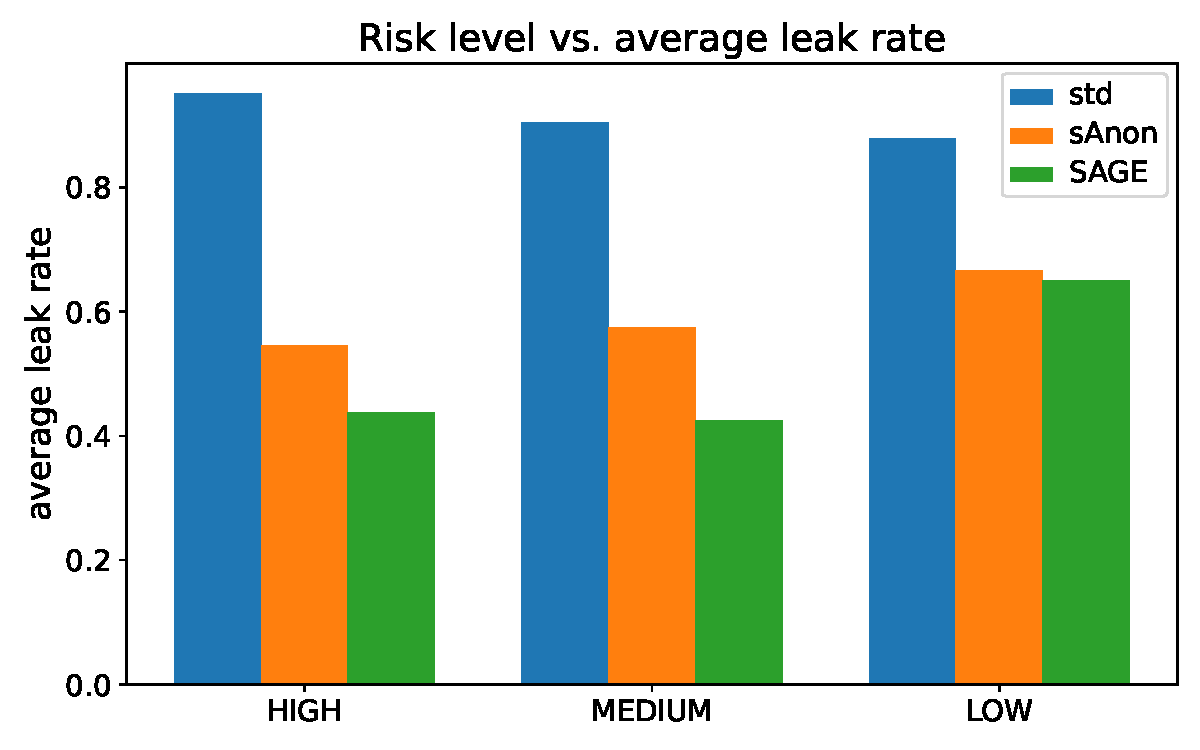
\includegraphics[width=0.7\textwidth]{figures/r1_precise_leak.pdf}
    \caption{Precise leakage rate}
    \label{evaluation-fig:precise_leakage}
\end{figure}  

\begin{figure}[h]
    \centering
    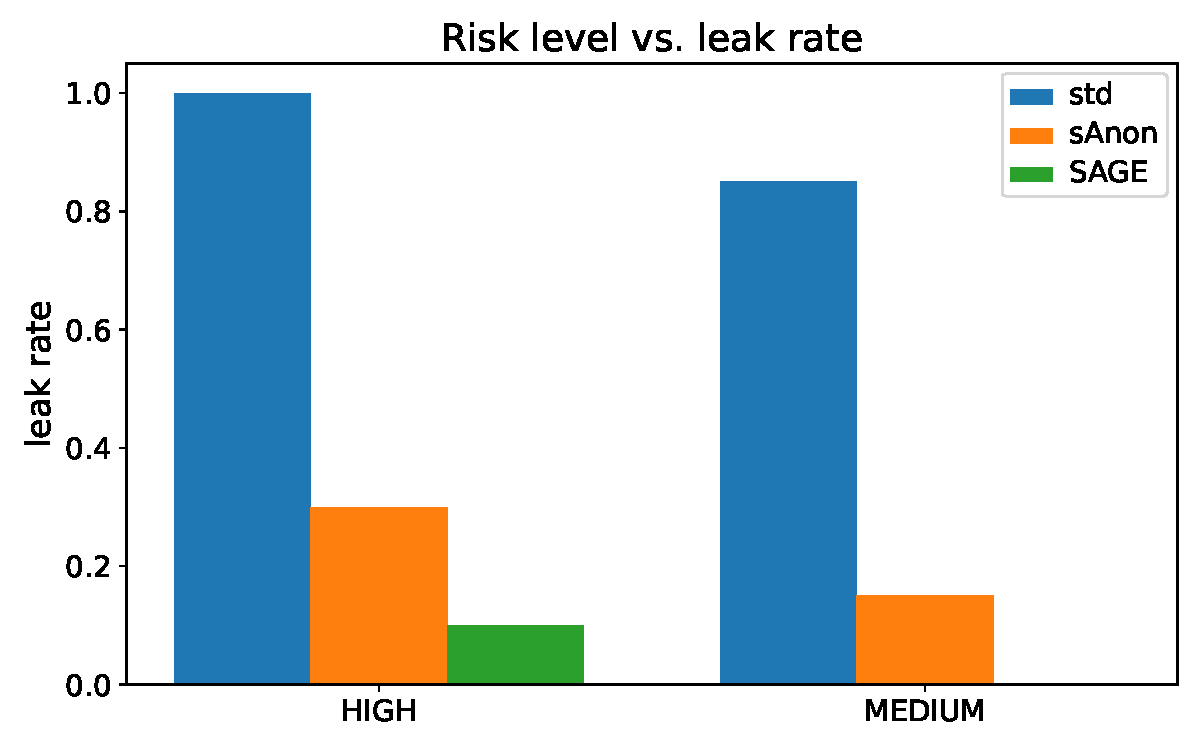
\includegraphics[width=0.7\textwidth]{figures/r1_leak_flag.pdf}
    \caption{Leakage rate for HIGH and MEDIUM clusters}
    \label{evaluation-fig:leakage_label}
\end{figure}  


\section{RQ3: Does selective anonymization preserve higher downstream utility than alternative privacy defenses while achieving comparable reductions in linkage risk?}

This research question investigates whether \textit{Selective Anonymization} preserves more downstream utility than alternative privacy-preserving pipelines, while still reducing privacy leakage. Utility is defined as the ability of a \ac{RAG} system to produce correct, complete and context-faithful answers to the benchmark questions described in Section \ref{evaluation-subsec:data-generation}.

\subsection{Experimental goal and expected results}
The primary goal is to compare the following three approaches regarding utility (see Section \ref{evaluation-subsec:baselines} for details):
\begin{enumerate}
\item \textbf{Default RAG:} retrieval over verbatim documents (upper-bound on utility, baseline for privacy).
\item \textbf{Synthetic Data (SAGE):} retrieval over synthetic documents, rewritten to remove identifying signals while keeping semantic content
\item \textbf{Selective Anonymization (ours):} retrieval over documents where only a subset of entities, selected by the policy described in Chapter \ref{chapter:approach}, are anonymized or removed.
% \item \textbf{Document-level Anonymization}: identical to \textbf{Sleective Anonymization}, but focusses only on the document level redaction and skips graph evaluation etc.
\end{enumerate}

We expect \textit{Default RAG} to achieve the highest utility across all question types, since no modifications are applied to the documents. \textit{SAGE} is expected to incur some loss in answer quality, particularly for specific questions, as attributes may be generalized or rewritten during synthesis. Finally, we expect \textit{Selective Anonymization} to strike a balance: achieving higher utility than \textit{SAGE}, particularly on general and multi-source questions, while still reducing leakage compared to \textit{Default RAG}.


\subsection{Scoring} 
We report three metrics to assess answer quality. All metrics are computed per question and then averaged across clusters and question types.
\paragraph{LLM-Judge Score} Each \ac{RAG}-system answer is evaluated by the automated \textit{LLM-Judge} (see Section \ref{evaluation-subsec:llm-judge}) which returns a scalar from $[0,1]$ with $1$ representing a perfect answer. The judge evaluates factual correctness and completeness relative to the optimal answer. A key advantage is that,  in contrast to string-based metrics,  semantically correct but differently phrased answers are not over-penalized.

\paragraph{ROUGE-1 Recall} To measure the lexical overlap between the generated and the optimal answer we use ROUGE-1 recall. Unlike ROUGE-L, which is sensitive to word order, ROUGE-1 captures token-level factual content more directly in our setting. Since the optimal answers are very short (often $\leq 15$ words), recall is preferred over F1: verbose but factually complete and correct answers should not be penalized simply for having low precision.

\paragraph{BERTScore Recall} We also report BERTScore Recall\cite{bertScore}, an automatic evaluation metric which computes a similarity score between each token in the generated answer and each token in the optimal answer using contextual embeddings. This makes BERTScore more robust towards paraphrasing than ROUGE, as it captures the semantic similarity instead of exact matches. However, it is less sensitive to minor factual errors (e.g. incorrect numbers or dates). Therefore it is used as a complementary rather than a standalone metric.


\subsection{Results}
sAnon delivers intermediate utility between standard RAG and SAGE across all metrics and question types. Its strongest retention is observable on general questions, while SAGE consistently scores the lowest. This aligns with the intended design trade-off of sAnon, which removes only a minimal set of entities, therefore preserving utiltiy particularly in non-senstiive contexts. 

\paragraph{LLM-Judge}
As expected, verbatim retrieval of standard RAG achieves the highest LLM-judge scores, establishing itself as an upper bound for answer quality \ref{evaluation-tab:utility-llm-details}. sAnon scores notably lower on specific questions, as identifying attributes of individuals are potentially masked. However, it retains relatively high utility on both single- and multi-source general questions. 
This suggests, that the value-level masking strategy maintains sufficient contextual and relational information between documents, including cases where non-sensitive cross-document reasoning is required. The low scores on specific questions are consistent with the privacy evaluation results, further demonstrating that sAnon is able to selectively redact information and break linkage in sensitive contexts.
In contrast, SAGE underperforms sAnon across all categories, with the largest gap on general questions, indicating that full synthetic replacements can harm utility even when privacy concerns are minimal.

\begin{table}[h!]
\centering
\caption{Detailed LLM-Judge Utility-Score across question types and baselines}
\label{evaluation-tab:utility-llm-details}
\begin{tabular}{l c c c}
\toprule
\textbf{(type/ source)} & \textbf{std\_RAG} & \textbf{sAnon} & \textbf{SAGE} \\
\midrule
specific / single & 0.796 & 0.222 & 0.144 \\
specific / multi & 0.560 & 0.253 & 0.158 \\
general / single & 0.869 & 0.655 & 0.444 \\
general / multi & 0.653 & 0.522 & 0.384 \\
\bottomrule
\end{tabular}
\end{table}


\paragraph{ROUGE1}
The ROUGE1-Recall results in Table \ref{evaluation-tab:utility-rouge-details} confirm the same general pattern. Standard RAG reaches the highest scores across all question types. sAnon achieves intermediate performance again, with stronger recall on general questions compared to specific ones. The relatively small gap between sAnon and standard RAG on general queries highlights that minimal masking largely preserves lexical overlap. SAGE exhibits the lowest recall across all categories, showing the disruptive effect of full text replacements on token-level similarity.

\begin{table}[h!]
\centering
\caption{Detailed ROUGE1-Recall Utility-Score across question types and baselines}
\label{evaluation-tab:utility-rouge-details}
\begin{tabular}{l c c c}
\toprule
\textbf{(type/ source)} & \textbf{std\_RAG} & \textbf{sAnon} & \textbf{SAGE} \\
\midrule
specific / single & 0.699 & 0.486 & 0.327 \\
specific / multi & 0.677 & 0.496 & 0.399 \\
general / single & 0.787 & 0.697 & 0.530 \\
general / multi & 0.688 & 0.598 & 0.485 \\
\bottomrule
\end{tabular}
\end{table}

\paragraph{BERT-Recall}
The BERT-Recall evaluation (Table~\ref{evaluation-tab:utility-bert-details}) provides a semantic perspective on utility. The trend observed in the previous measures persists with scores decreasing from standard RAG to sAnon to SAGE. sAnon preserves comparatively high semantic similarity on general questions, leading to the conclusion that minimal masking is less disruptive for non-private contexts. Unsurprisingly, the full substitution performed by SAGE also reduces semantic similarity to the original text and answer


\begin{table}[h!]
\centering
\caption{Detailed BERT-Recall Utility-Score across question types and baselines}
\label{evaluation-tab:utility-bert-details}
\begin{tabular}{l c c c}
\toprule
\textbf{(type/ source)} & \textbf{std\_RAG} & \textbf{sAnon} & \textbf{SAGE} \\
\midrule
specific / single & 0.537 & 0.303 & 0.201 \\
specific / multi & 0.419 & 0.251 & 0.207 \\
general / single & 0.605 & 0.510 & 0.365 \\
general / multi & 0.416 & 0.345 & 0.264 \\
\bottomrule
\end{tabular}
\end{table}